%%%%%%%%%%%%%%%%%%%%%%%%%%%%%%%%%%%%%%%%%%%%%%%%%%%%%%%%%%%%%%%%%%%%%%%%%%
% Conference extended abstract -- Utah AI Convergence
% Plain-language, "better poster"-style companion to the full Digital
% Discovery manuscript (paper/main.tex). This is a SEPARATE draft from the
% journal paper; it is deliberately short, jargon-free, and focused on the
% generative-AI case study rather than on the powder-dosing problem itself.
%%%%%%%%%%%%%%%%%%%%%%%%%%%%%%%%%%%%%%%%%%%%%%%%%%%%%%%%%%%%%%%%%%%%%%%%%%%

\documentclass[11pt]{article}

\usepackage[letterpaper,margin=2cm]{geometry}
\usepackage[T1]{fontenc}
\usepackage{lmodern}
\usepackage{graphicx}
\usepackage{microtype}
\usepackage{titlesec}
\usepackage{parskip}
\usepackage[colorlinks=true,allcolors=blue]{hyperref}
\usepackage{caption}
\captionsetup{font=small,labelfont=bf}

\graphicspath{{../figures/}}

\titleformat{\section}{\large\bfseries}{}{0pt}{}
\titlespacing*{\section}{0pt}{10pt}{4pt}
\setlength{\parskip}{6pt}

\pagestyle{empty}

\begin{document}

\begin{center}
  {\LARGE\bfseries We built a lab instrument without CAD software---%
  artificial intelligence designed every part}\\[6pt]
  {\large An open-source, 3D-printed powder doser as a case study in
  AI-assisted hardware design}\\[8pt]
  {\normalsize Sam Charles, Will Mulberry, Luke Winters, Carl Robinson,
  Gage Erickson, and Sterling G. Baird}\\[2pt]
  {\small Brigham Young University \quad\textbar\quad University of Utah}\\[2pt]
  {\small Conference extended abstract --- Utah AI Convergence}
\end{center}

\vspace{4pt}
\noindent\fbox{\parbox{\dimexpr\linewidth-2\fboxsep-2\fboxrule}{%
  \textbf{In one sentence:} We used generative AI to design a working
  laboratory machine from start to finish, and the most important result is
  not the machine itself---it is what we learned about letting AI do the
  engineering.}}

\section{Background}

Modern research labs increasingly run experiments automatically, with robots
mixing chemicals and machine-learning software deciding what to try next.
These ``self-driving labs'' are good at handling liquids but still struggle
with powders, which most labs weigh out by hand. Machines that dose powders
automatically do exist, but they cost tens of thousands of dollars, putting
them out of reach for most academic groups.

At the same time, AI tools that can write code and even generate 3D shapes
are improving quickly. We wanted to know a practical question: can today's AI
actually design a real, physical, working instrument---not just a shape on a
screen---if a small team guides it? To find out, we set ourselves a strict
rule and a real goal.

\section{Design solution}

The goal was a low-cost powder doser that any lab could 3D-print and build.
Our design uses a turning screw (an auger) to push powder out a nozzle, a
small tapping and vibrating mechanism to keep the powder flowing, a tilting
base so the powder always lands in the same spot, and a precise balance that
weighs the powder as it falls and tells the machine when to stop. A \$6
microcontroller runs everything. One complete unit can be built for under
\$200, roughly one hundred times cheaper than commercial systems.

For this conference the machine is mainly an example. The point we want to
make is not that it dispenses powder well, but that it was designed in an
unusual way.

\begin{figure}[t]
  \centering
  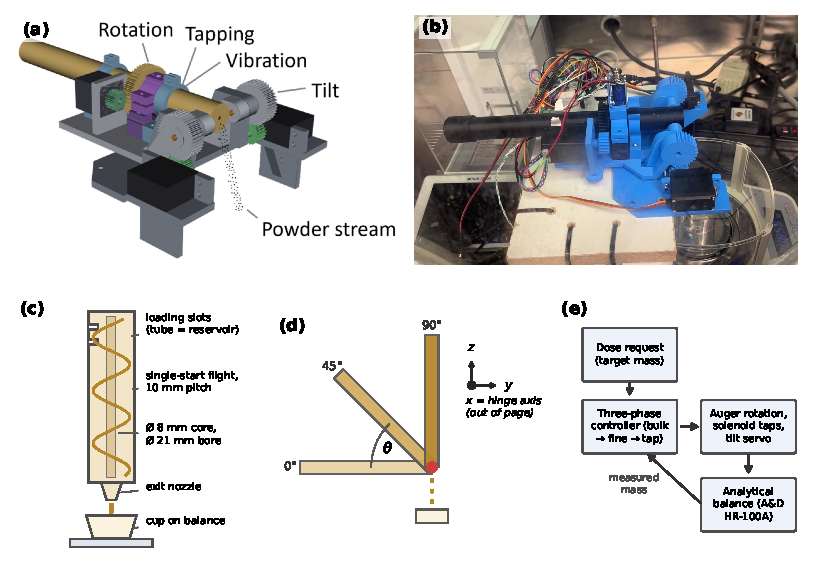
\includegraphics[width=0.92\linewidth]{fig1_overview}
  \caption{The powder doser. Humans chose the overall design and reviewed,
  printed, and tested every part; AI tools created the 3D models. No
  traditional CAD software was used.}
  \label{fig:overview}
\end{figure}

\section{Generative AI}

Here is the strict rule we followed: \textbf{no traditional CAD software was
used at any point.} Engineers normally design parts by hand in programs like
SolidWorks or Fusion~360. We never opened them. Instead, every part was made
by AI.

We worked in two ways. Most parts were built by AI ``coding agents'' that
write the design as computer code; the code is turned into a 3D model and a
picture automatically, and our team reviewed each result and asked for fixes.
Late in the project we also used Zoo Design Studio and its AI agent,
Zookeeper, which we drove almost entirely by typing instructions in plain
language rather than by drawing.

Two lessons stood out. First, \textbf{asking the AI to design the whole
machine at once did not work}---the parts overlapped, floated in mid-air, or
left no room for the motors. But \textbf{asking for one part at a time, with
clear instructions about how it connects to its neighbors, worked well.}
Second, \textbf{the AI needed constant checking.} It would sometimes quietly
change a part we had already finished, so every new version had to be
re-inspected. Automated checks and careful human review caught most problems.

We were honest about the trade-offs. An experienced engineer using normal CAD
software would have been faster and produced cleaner parts. What the AI
approach gave us instead was a complete, written record of every decision,
every prompt, and every mistake. That record makes the whole project
reproducible and easy for others to learn from---something a normal CAD
session leaves behind only in a designer's head.

\section{Conclusion and future work}

We designed and built a real, working laboratory instrument entirely with
generative AI, under human direction, and without ever touching conventional
CAD software. The honest, complete history of the project---including its
failures---is public, so it doubles as a case study of what AI can and cannot
yet do in hardware design.

Next, we are extending the design into a multi-powder version, adding
automatic calibration, and continuing to test new AI design tools. Every
design file, the firmware, and the full log of AI prompts and responses are
freely available at
\url{https://github.com/vertical-cloud-lab/powder-doser}.

\end{document}
